
\documentclass[11pt]{article}
\usepackage[margin=1.3in]{geometry}
\usepackage{hyperref}
\usepackage{multirow}
\usepackage{booktabs}
\usepackage{epsdice}

\usepackage{../maybe}

\newcommand{\command}[1]{\text{\textbackslash}\texttt{#1}}
\newcommand{\param}[1]{\{\text{$\langle$}\texttt{#1}\text{$\rangle$}\}}
\newcommand{\optparam}[1]{[\text{$\langle$}\texttt{#1}\text{$\rangle$}]}


\begin{document}

\section{Motivation}
This package is meant to simplify and streamline many of the basic tools in probability theory and statistics, such as Venn diagrams, histograms, point mass functions, and such.
It relies heavily on \texttt{TikZ}.

\section{Configuration}
To prevent side-effects of asymmetric scaling when using \texttt{xscale} and \texttt{yscale} options of the \texttt{tikzpicture} environment (e.g., circles will may be stretched and become ellipses), this package implements its own scaling system.

It may be reset to the default unit scale by using the
\[
    \command{mayberesetscale}
\]
command (no arguments), or set to an arbitrary value by using the
\[
    \command{maybesetscale}\param{xscale}\param{yscale}
\]
command.
Setting the scale to negative value(s) achieves reflection.

The current values of the scales may be retrieved through the \command{maybexscale} and \command{maybeyscale} commands that take no arguments.

%Certain measurements ignore internal scaling (up to the sign of the scale to respect reflection).
%They are referenced in this document as ``absolute'', and marked with \texttt{\Absolute}.


\section{Styling}
Each command utilizing TikZ has options for styling.
Some are specific to a particular command, while others are universal.
Whenever there are labels (nodes) involved, one could use
\[
    \command{maybesetnodestyle}\param{style}
\]
to set or override the style of the node(s).


To prevent accidents while mixing pure numbers and units in TiKZ, every option that ignores \command{maybexscale} and \command{maybeyscale} is implemented through \texttt{xshift} and \texttt{yshift}, respectively.


\section{Axes}
Drawing an axis may be achieved by either
\[
    \command{maybeHAxis}\optparam{label}\param{xcoordinates}\param{ylocation},
\]
which produces a horizontal axis with an optional label, or
\[
    \command{maybeVAxis}\optparam{label}\param{ycoordinates}\param{xlocation}.
\]
In each case the \texttt{coordinates} have to be a comma-separated list, and the axis will run from $\min(\texttt{coordinates})$ to $\max(\texttt{coordinates})$.
The line will be extended by the absolute amount (not affected by \command{maybexscale} or \command{maybeyscale}), which is defined by
\[
    \command{maybe$@$xaxisextendfrom}, \command{maybe$@$xaxisextendto}
\]
for the horizontal axis, and
\[
    \command{maybe$@$yaxisextendfrom}, \command{maybe$@$yaxisextendto}
\]
for the vertical axes.

\begin{center}
    \begin{tikzpicture}
        \maybesetscale{0.45}{1}
        \maybeHAxis[$X$]{17, 29}{0};
    \end{tikzpicture}
    \\
    \begin{tikzpicture}
        \maybesetscale{-0.45}{-1}
        \maybeHAxis[$X$]{17, 29}{0};
    \end{tikzpicture}
\end{center}

\begin{center}
    \begin{tikzpicture}
        \maybesetscale{1}{0.1}
        \maybeVAxis[$Y$]{17, 29}{0};
    \end{tikzpicture}
    \hspace{2em}
    \begin{tikzpicture}
        \maybesetscale{-1}{-0.1}
        \maybeVAxis[$Y$]{17, 29}{0};
    \end{tikzpicture}
\end{center}

The style of the axis may be changed by calling the \command{maybesetaxisstyle} command.
\begin{center}
    \begin{tikzpicture}
        \maybesetscale{0.5}{1}
        \maybesetaxisstyle{thick, >={Latex}}
        \maybeHAxis[$X$]{17, 29}{0};
    \end{tikzpicture}
\end{center}


\paragraph*{Axis labels and ticks.}
To add labels/ticks to the horizontal or vertical axis, use the
\begin{align*}
    &\command{maybeHLabels}\optparam{xlabels}\param{xcoordinates}\param{ylocation} \\
    &\command{maybeHTicks}\param{xcoordinates}\param{ylocation}
\end{align*}
or
\begin{align*}
    &\command{maybeVLabels}\optparam{ylabels}\param{ycoordinates}\param{xlocation} \\
    &\command{maybeVTicks}\param{ycoordinates}\param{xlocation}
\end{align*}
commands, respectively.
Labels default to the coordinates specified.
Tick position may be changed by calling \command{maybeticksabove}, \command{maybeticksbelow}, or \command{maybetickscenter}.

\begin{center}
    \begin{tikzpicture}
        \maybesetscale{0.45}{1}
        \maybeHAxis[$X$]{17, 29}{0};
        \maybeHLabels{20, 25}{0};
        \maybeHTicks{20, 25}{0};
    \end{tikzpicture}
    \\
    \begin{tikzpicture}
        \maybesetscale{-0.45}{-1}
        \maybeHAxis[$X$]{17, 29}{0};
        \maybeHLabels{20, 25}{0};
        \maybeHTicks{20, 25}{0};
    \end{tikzpicture}
\end{center}

\begin{center}
    \begin{tikzpicture}
        \maybesetscale{1}{0.1}
        \maybeVAxis[$Y$]{17, 29}{0};
        \maybeVLabels{20, 25}{0};
        \maybeVTicks{20, 25}{0};
    \end{tikzpicture}
    \hspace{2em}
    \begin{tikzpicture}
        \maybesetscale{-1}{-0.1}
        \maybeVAxis[$Y$]{17, 29}{0};
        \maybeVLabels{20, 25}{0};
        \maybeVTicks{20, 25}{0};
    \end{tikzpicture}
\end{center}

\section{Visualizing Data}
\paragraph*{Point mass functions.}
To add vertical or horizontal bars to a graph, use the
\[
    \command{maybeVBars}\optparam{barlabels}\param{xcoordinates}\param{barlengths}\param{ylocation}
\]
or
\[
    \command{maybeHBars}\optparam{barlabels}\param{ycoordinates}\param{barlengths}\param{xlocation}
\]
commands, respectively.
Labels default to the lengths specified.


\begin{center}
    \begin{tikzpicture}
        \maybesetscale{0.45}{1}
        \maybeHAxis[$X$]{17, 29}{0};
        \maybeHLabels{20, 25}{0};
        \maybeVBars["3/4", "1/4"]{20, 25}{0.75, 0.25}{0};
    \end{tikzpicture}
    \\
    \begin{tikzpicture}
        \maybesetscale{-0.45}{-1}
        \maybeHAxis[$X$]{17, 29}{0};
        \maybeHLabels{20, 25}{0};
        \maybeHTicks{20, 25}{0};
        \maybeVBars["3/4", "1/4"]{20, 25}{0.75, 0.25}{0};
    \end{tikzpicture}
\end{center}

\begin{center}
    \begin{tikzpicture}
        \maybesetscale{2}{0.2}
        \maybeVAxis[$Y$]{17, 29}{0};
        \maybeVLabels{20, 25}{0};
        \maybeHBars["3/4", "1/4"]{20, 25}{0.75, 0.25}{0};
    \end{tikzpicture}
    \hspace{2em}
    \begin{tikzpicture}
        \maybesetscale{-2}{-0.2}
        \maybeVAxis[$Y$]{17, 29}{0};
        \maybeVLabels{20, 25}{0};
        \maybeVTicks{20, 25}{0};
        \maybeHBars["3/4", "1/4"]{20, 25}{0.75, 0.25}{0};
    \end{tikzpicture}
\end{center}

\paragraph*{Histograms.}
To add a vertical or horizontal histogram rectangle to a graph, use the
\[
    \command{maybeVHistBar}\optparam{label}\param{xcoordinates}\param{ylocation}\param{area}
\]
or
\[
    \command{maybeHHistBar}\optparam{label}\param{ycoordinates}\param{xlocation}\param{area}
\]
commands, respectively.
Label defaults to the area specified.

\begin{center}
    \begin{tikzpicture}
        \maybesetscale{0.45}{10.0}
        \maybeHAxis[$X$]{17, 29}{0};
        \maybeHLabels{20, 25}{0};
        \maybeVHistBar{20, 25}{0}{0.25};
    \end{tikzpicture}
    \\
    \begin{tikzpicture}
        \maybesetscale{-0.45}{-10.0}
        \maybeHAxis[$X$]{17, 29}{0};
        \maybeHLabels{20, 25}{0};
        \maybeVHistBar{20, 25}{0}{0.25};
    \end{tikzpicture}
\end{center}

\begin{center}
    \begin{tikzpicture}
        \maybesetscale{6.0}{0.28}
        \maybeVAxis[$Y$]{17, 29}{0};
        \maybeVLabels{20, 25}{0};
        \maybeHHistBar{20, 25}{0}{0.25};
    \end{tikzpicture}
    \hspace{2em}
    \begin{tikzpicture}
        \maybesetscale{-6.0}{-0.28}
        \maybeVAxis[$Y$]{17, 29}{0};
        \maybeVLabels{20, 25}{0};
        \maybeHHistBar{20, 25}{0}{0.25};
    \end{tikzpicture}
\end{center}

\paragraph*{Box-plots.}
To add a horizontal or vertical box-plot to a graph, use the
\[
    \command{maybeHBoxPlot}\param{min, Q1, Q2, Q3, max}\param{ylocation}\param{height}
\]
or
\[
    \command{maybeVBoxPlot}\param{min, Q1, Q2, Q3, max}\param{xlocation}\param{width}
\]
commands, respectively.

\begin{center}
    \begin{tikzpicture}
        \maybesetscale{0.45}{10.0}
        \maybeHAxis[$X$]{17, 29}{0};
        \maybeHLabels{20, 25}{0};
        \maybeHTicks{20, 25}{0};
        \maybeHBoxPlot{17, 20, 21, 25, 29}{0.07}{0.07};
    \end{tikzpicture}
    \\
    \begin{tikzpicture}
        \maybesetscale{-0.45}{-10.0}
        \maybeHAxis[$X$]{17, 29}{0};
        \maybeHLabels{20, 25}{0};
        \maybeHTicks{20, 25}{0};
        \maybeHBoxPlot{17, 20, 21, 25, 29}{0.07}{0.07};
    \end{tikzpicture}
\end{center}

\begin{center}
    \begin{tikzpicture}
        \maybesetscale{12.0}{0.28}
        \maybeVAxis[$Y$]{17, 29}{0};
        \maybeVLabels{20, 25}{0};
        \maybeVTicks{20, 25}{0};
        \maybeVBoxPlot{17, 20, 21, 25, 29}{0.07}{0.07};
    \end{tikzpicture}
    \hspace{2em}
    \begin{tikzpicture}
        \maybesetscale{-12.0}{-0.28}
        \maybeVAxis[$Y$]{17, 29}{0};
        \maybeVLabels{20, 25}{0};
        \maybeVTicks{20, 25}{0};
        \maybeVBoxPlot{17, 20, 21, 25, 29}{0.07}{0.07};
    \end{tikzpicture}
\end{center}


\section{Dice}
This package provides a TiKZ-based alternative to \texttt{epsdice}.

\begin{center}
    \newcommand{\noepsdice}{\phantom{\epsdice{1}}}
    \newcommand{\epsdicecommand}[1]{\command{epsdice}\{\texttt{#1}\}}
    \newcommand{\maybedicecommand}[1]{\command{maybedice}\{\texttt{#1}\}}
    \begin{tabular}{@{} l c @{}}
        \toprule
        \texttt{maybedice} command  & output of \texttt{epsdice} / \texttt{maybedice} / \texttt{maybevardice}  \\ \midrule
        \maybedicecommand{1}        & \epsdice{1} / \maybedice{1} / \maybevardice{1} \\
        \maybedicecommand{2}        & \epsdice{2} / \maybedice{2} / \maybevardice{2} \\
        \maybedicecommand{3}        & \epsdice{3} / \maybedice{3} / \maybevardice{3} \\
        \maybedicecommand{4}        & \epsdice{4} / \maybedice{4} / \maybevardice{4} \\
        \maybedicecommand{5}        & \epsdice{5} / \maybedice{5} / \maybevardice{5} \\
        \maybedicecommand{6}        & \epsdice{6} / \maybedice{6} / \maybevardice{6} \\
        \maybedicecommand{7}        & \noepsdice\ / \maybedice{7} / \maybevardice{7} \\
        \maybedicecommand{8}        & \noepsdice\ / \maybedice{8} / \maybevardice{8} \\
        \maybedicecommand{9}        & \noepsdice\ / \maybedice{9} / \maybevardice{9} \\
        \bottomrule
    \end{tabular}
\end{center}


\end{document}
